\documentclass[12pt,a4paper]{article}
\usepackage[a4paper, margin=0.8in, headheight=14pt]{geometry}
\usepackage{fontspec}
\usepackage{unicode-math}
\setmainfont{TeX Gyre Pagella}
\setmonofont[Scale=0.88]{TeX Gyre Cursor}
\setmathfont{Latin Modern Math}
\usepackage{xcolor}
\usepackage{colortbl}
\usepackage{titlesec}
\usepackage{enumitem}
\usepackage{tabularx}
\usepackage{booktabs}
\usepackage{array}
\usepackage{amsmath}
\usepackage{tikz}
\usetikzlibrary{shapes.geometric, arrows.meta, positioning, calc, fit, decorations.pathreplacing, decorations.pathmorphing, patterns, backgrounds}
\usepackage[american]{circuitikz}
\usepackage{tcolorbox}
\tcbuselibrary{skins, breakable}
\usepackage{etoolbox}
\usepackage{hyperref}
\usepackage{fancyhdr}
\usepackage{graphicx}
\usepackage{microtype}
\hyphenpenalty=10000
\exhyphenpenalty=10000
\sloppy
\usepackage{caption}
\usepackage{setspace}
\usepackage{multirow}
\usepackage{tocloft}
\newcommand{\Q}[2]{\item \textbf{#1}\par #2 \vspace{4pt}}
\definecolor{myred}{RGB}{196,30,58}       % section headings
\definecolor{mydark}{RGB}{30,30,50}       % body text
\definecolor{mygreen}{RGB}{14,120,80}     % definition boxes
\definecolor{myteal}{RGB}{0,130,140}      % formula boxes, diagrams, subsection headings
\definecolor{myamber}{RGB}{180,100,0}     % example boxes
\definecolor{mypurple}{RGB}{100,30,160}   % exam/viva boxes
\definecolor{myblue}{RGB}{25,90,170}      % hyperlinks/diagrams
\definecolor{mygray}{RGB}{246,247,249}    % tikzbox background
\definecolor{mgframe}{RGB}{180,185,200}   % tikzbox border
\definecolor{watermark}{RGB}{145,150,170} % footer watermark
\definecolor{hdrred}{RGB}{250,232,235}
\definecolor{hdrgreen}{RGB}{220,244,233}
\definecolor{hdrteal}{RGB}{220,242,244}
\definecolor{hdramber}{RGB}{253,242,215}
\definecolor{hdrpurple}{RGB}{238,228,255}
\definecolor{hdrblue}{RGB}{235,242,250}
\AfterEndEnvironment{tcolorbox}{\color{mydark}}

\titleformat{\section}{\large\bfseries\color{myred}}{\thesection.}{0.5em}{}[\vspace{1pt}{\color{myred}\rule{\linewidth}{0.8pt}}]
\titleformat{\subsection}{\normalsize\bfseries\color{myteal}}{\thesubsection}{0.5em}{}
\titlespacing*{\section}{0pt}{18pt}{7pt}
\titlespacing*{\subsection}{0pt}{11pt}{4pt}
\setlength{\parindent}{0pt}
\setlength{\parskip}{4pt}
\renewcommand{\cfttoctitlefont}{\large\bfseries\color{myred}}
\renewcommand{\cftaftertoctitle}{\par\noindent{\color{myred}\rule{\linewidth}{0.8pt}}}
\setlength{\cftbeforetoctitleskip}{0pt}
\setlength{\cftaftertoctitleskip}{6pt}
\renewcommand{\cftsecfont}{\normalsize\bfseries\color{mydark}}
\renewcommand{\cftsecpagefont}{\normalsize\bfseries\color{mydark}}
\renewcommand{\cftsecleader}{\cftdotfill{\cftdotsep}}
\setlength{\cftbeforesecskip}{7pt}
\renewcommand{\cftsubsecfont}{\small\color{mydark}}
\renewcommand{\cftsubsecpagefont}{\small\color{mydark}}
\setlength{\cftbeforesubsecskip}{3pt}
\setlength{\cftsubsecindent}{1.4em}
\renewcommand{\cftpartfont}{\normalsize\bfseries\color{myteal}}
\renewcommand{\cftpartpagefont}{\normalsize\bfseries\color{myteal}}
\setlength{\cftbeforepartskip}{14pt}
\renewcommand{\arraystretch}{1.45}
\setlength{\tabcolsep}{6pt}
\arrayrulecolor{mydark}
\newcolumntype{B}[1]{>{\small\bfseries\raggedright\arraybackslash}m{#1}}
\newcolumntype{C}[1]{>{\centering\arraybackslash}m{#1}}
\newcolumntype{Y}{>{\small\raggedright\arraybackslash}X}
\renewcommand{\tabularxcolumn}[1]{m{#1}}
\newcommand{\currmodule}{Module 1}
\pagestyle{fancy}
\fancyhf{}
\fancyhead[L]{\small\color{myred}\textbf{OE-EC804C}\;\color{mydark}--- Organizational Behavior}
\fancyhead[R]{\small\color{myteal}\textbf{\currmodule\ Notes}}
\fancyfoot[C]{\small\color{mydark}\thepage}
\fancyfoot[R]{\small\color{watermark}\textit{\copyright\ Biraj}}
\renewcommand{\headrulewidth}{0.5pt}
\renewcommand{\footrulewidth}{0.3pt}

\hypersetup{colorlinks=true, linkcolor=myteal, urlcolor=myteal,
  pdfauthor={Biraj Sarkar},
  pdftitle={OE-EC804C --- Combined Notes}}

\tcbset{
  tikzbox/.style={colback=mygray, colframe=mgframe, boxrule=0.6pt, arc=4pt,
    left=8pt, right=8pt, top=6pt, bottom=6pt,
    colbacktitle=mgframe, coltitle=mydark, fonttitle=\small\bfseries},
  defbox/.style={colback=hdrgreen, colframe=mygreen, boxrule=0.8pt, arc=4pt,
    left=9pt, right=9pt, top=6pt, bottom=6pt,
    colbacktitle=mygreen, coltitle=white, fonttitle=\small\bfseries},
  formulabox/.style={colback=hdrteal, colframe=myteal, boxrule=0.8pt, arc=4pt,
    left=9pt, right=9pt, top=7pt, bottom=7pt,
    colbacktitle=myteal, coltitle=white, fonttitle=\small\bfseries},
  examplebox/.style={colback=hdramber, colframe=myamber, boxrule=0.8pt, arc=4pt,
    left=9pt, right=9pt, top=6pt, bottom=6pt,
    colbacktitle=myamber, coltitle=white, fonttitle=\small\bfseries},
  masonbox/.style={colback=hdrpurple, colframe=mypurple, boxrule=0.8pt, arc=4pt,
    left=9pt, right=9pt, top=6pt, bottom=6pt,
    colbacktitle=mypurple, coltitle=white, fonttitle=\small\bfseries},
  exambox/.style={colback=hdrpurple, colframe=mypurple, boxrule=1pt, arc=5pt,
    left=10pt, right=10pt, top=8pt, bottom=8pt,
    colbacktitle=mypurple, coltitle=white, fonttitle=\bfseries,
    title after break={\textbf{Frequently Asked / Viva Questions (contd.)}}}
}
\tcbset{breakable}
\tcbset{coltext=mydark}
\tcbset{after={\color{mydark}}}

\tikzset{
  line/.style={draw=mydark, thick},
  arrow/.style={draw=mydark, -{Stealth[scale=1.2]}, thick},
  block/.style={draw=myteal, fill=hdrteal, rectangle, rounded corners=3pt, align=center, font=\small\bfseries, minimum height=0.8cm, text width=2.4cm},
  sblock/.style={draw=mypurple, fill=hdrpurple, rectangle, rounded corners=3pt, align=center, font=\small\bfseries, minimum height=0.8cm, text width=2.2cm}
}

\newcommand{\modulestart}[2]{%
  \clearpage
  \renewcommand{\currmodule}{Module #1}%
  \renewcommand{\theHsection}{mod#1.\arabic{section}}%
  \renewcommand{\theHsubsection}{\theHsection.\arabic{subsection}}%
  \renewcommand{\theHsubsubsection}{\theHsubsection.\arabic{subsubsection}}%
  \phantomsection
  \addcontentsline{toc}{part}{Module #1: #2}%
  \setcounter{section}{0}%
  \begin{center}
    \vspace*{1.0cm}
    {\Huge\bfseries\color{myred} Module #1}\\[10pt]
    {\Large\bfseries\color{mydark} #2}\\[10pt]
    {\color{myred}\rule{0.55\linewidth}{1.2pt}}
  \end{center}
  \vspace{14pt}
}
\begin{document}

\thispagestyle{empty}

% ─── Page Border (TikZ Overlay) ────────────────────────────────────────────────
\begin{tikzpicture}[remember picture, overlay]
  % Outer border (fine line in mgframe)
  \draw[color=mgframe, line width=1.5pt] 
    ($(current page.north west) + (0.6in, -0.6in)$) rectangle 
    ($(current page.south east) + (-0.6in, 0.6in)$);
  % Inner border (finer accent line in myred)
  \draw[color=myred, line width=0.8pt] 
    ($(current page.north west) + (0.65in, -0.65in)$) rectangle 
    ($(current page.south east) + (-0.65in, 0.65in)$);
\end{tikzpicture}

\vspace*{1.0cm}
\begin{center}
  {\Huge\bfseries\color{myred} OE-EC804C}\\[10pt]
  {\LARGE\bfseries\color{mydark} Organizational Behavior}\\[20pt]
  {\color{myred}\rule{0.7\linewidth}{1.5pt}}\\[18pt]
  {\Large\color{myteal}\textbf{Combined Module Notes}}\\[8pt]
  {\large\color{mydark} Modules 1 -- 4}\\[40pt]
  {\normalsize\color{mydark} Semester}\\[12pt]
  {\normalsize\color{mydark} CGEC \;$|$\; B.Tech ECE (2023--27)}
\end{center}
\vspace{1.0cm}
\begin{center}
  \begin{tcolorbox}[colback=mygray, colframe=mgframe, boxrule=0.5pt, arc=3pt, width=0.85\linewidth]
    \centering\small\color{mydark}
    \textbf{Disclaimer / Study Guide Notice:}\\
    These are condensed \textbf{Short Notes} focusing on core theory, key formulas, block/circuit diagrams, and standard viva Q\&As for university exam revision. Exhaustive numerical practice problems and derivation edge cases are not covered. This serves as a quick-revision reference guide for students.
  \end{tcolorbox}
\end{center}
\vfill
\vspace{0.6cm}
\begin{center}
  {\large\bfseries\color{mypurple} Biraj Sarkar}\\[16pt]
  {\footnotesize\color{watermark}\textbf{IN ASSOCIATION WITH}}\\[8pt]
  {\small\bfseries\color{mydark} MAKAUT Wingman \quad$\bullet$\quad MAKAUT Future Minds}\\[12pt]
  {\large\bfseries\color{myteal} Cooch Behar Government Engineering College}
\end{center}
\vfill
\begin{center}{\small\color{watermark}\textit{Exam-Ready Notes}}\end{center}
\clearpage

\hypersetup{linkcolor=mydark}
\tableofcontents
\hypersetup{linkcolor=myteal}
\clearpage

% -- Module 1 -----------------------------------------------------------------
\modulestart{1}{Meaning and Definition of Organization}

\section{Meaning and Definition of Organization}

An \textbf{Organization} is a structured social entity consisting of a group of people working together in a coordinated manner to achieve specific, pre-determined organizational goals and objectives.

\begin{tcolorbox}[defbox, title={Definition of Organization}]
  An \textbf{Organization} is a consciously coordinated social unit, composed of two or more people, that functions on a relatively continuous basis to achieve a common goal or set of goals (Stephen P. Robbins).
\end{tcolorbox}

\subsection{Key Components of an Organization}
Every modern engineering or corporate organization comprises four essential elements:
\begin{enumerate}[leftmargin=*, itemsep=4pt]
  \item \textbf{People:} The human resource (employees, managers, leaders) who form the internal social system.
  \item \textbf{Structure:} The formal relationships, roles, hierarchy, and division of authority that dictate how work is divided and coordinated.
  \item \textbf{Technology:} The physical tools, machinery, software algorithms, processes, and techniques used to transform inputs into outputs.
  \item \textbf{Environment:} The external political, economic, social, technological, legal, and ecological (PESTLE) forces operating outside the organizational boundary.
\end{enumerate}

\subsection{Formal vs. Informal Organizations}
Organizations operate through two parallel structural dimensions:

\par\vspace{6pt}\noindent
\begingroup
\setlength{\tabcolsep}{5pt}%
\setlength{\extrarowheight}{3pt}%
\renewcommand{\arraystretch}{1.35}%
\begin{tabularx}{\linewidth}{|>{\raggedright\arraybackslash\bfseries}p{3.5cm}|Y|Y|}
\hline
\multicolumn{1}{|c|}{\textbf{Feature}} & \multicolumn{1}{c|}{\textbf{Formal Organization}} & \multicolumn{1}{c|}{\textbf{Informal Organization}} \\
\hline
Origin \& Creation & Deliberately established by top management via official policies \& org charts. & Spontaneously formed by employees based on personal relationships \& common interests. \\
\hline
Structure & Well-defined, rigid hierarchy of authority and delegated positions. & Unstructured, flexible, and fluid social network. \\
\hline
Communication Channel & Official channels (chain of command, memo, email protocols). & Unofficial channel (grapevine, social chatter, coffee breaks). \\
\hline
Primary Focus & Goal achievement, productivity, efficiency, and task execution. & Individual social satisfaction, belongingness, and emotional support. \\
\hline
Leadership & Appointed managers with legitimate positional power. & Natural/informal leaders emerging from group acceptance and charisma. \\
\hline
\end{tabularx}
\endgroup

% ===============================================================================
% 2. FEATURES AND PRINCIPLES OF ORGANIZATION
% ===============================================================================
\section{Features and Principles of Organization}

\subsection{Key Features of an Organization}
\begin{itemize}[leftmargin=*, itemsep=4pt]
  \item \textbf{Division of Labor:} Complex tasks are broken down into specialized jobs to optimize productivity.
  \item \textbf{Hierarchy of Authority:} A scalar chain of command defining superior-subordinate reporting lines.
  \item \textbf{Common Objectives:} Alignment of individual and departmental activities toward overarching organizational goals.
  \item \textbf{Coordination:} Systematic integration of diverse departmental efforts to eliminate redundancy.
  \item \textbf{Continuity \& Permanence:} Designed to exist beyond the tenure of individual founders or employees.
\end{itemize}

\subsection{Henri Fayol's Principles of Management / Organization}
Classical administrative theory, articulated by \textbf{Henri Fayol}, lays down fundamental principles for organizing enterprises:

\begin{tcolorbox}[formulabox, title={Core Administrative Principles (Fayol)}]
  \begin{enumerate}[leftmargin=*, itemsep=3pt]
    \item \textbf{Division of Work:} Specialization increases output by making employees more efficient.
    \item \textbf{Authority \& Responsibility:} Right to give orders backed by obligation to answer for outcomes.
    \item \textbf{Unity of Command:} Each subordinate receives orders from \textbf{one and only one} superior.
    \item \textbf{Unity of Direction:} One head and one plan for a group of activities having the same objective.
    \item \textbf{Scalar Chain:} The unbroken chain of authority extending from top executive to lowest level.
    \item \textbf{Span of Control:} The optimal number of subordinates a manager can directly supervise effectively.
  \end{enumerate}
\end{tcolorbox}

% ===============================================================================
% 3. ORGANIZATIONAL STRUCTURES
% ===============================================================================
\section{Organizational Structures}

An \textbf{Organizational Structure} defines how tasks are formally divided, grouped, and coordinated across departments and management levels.

\subsection{Types of Organizational Structures}

\begin{enumerate}[leftmargin=*, itemsep=5pt]
  \item \textbf{Functional Structure:} Grouping employees into departments based on specialized skills/functions (e.g., R\&D, Engineering, Marketing, Finance, HR).
  \item \textbf{Divisional Structure:} Self-contained units organized around products, geographic regions, or customer segments.
  \item \textbf{Matrix Structure:} A dual-authority structure combining functional departments with project/product teams. Employees report to both a Functional Manager and a Project Manager.
  \item \textbf{Line and Staff Structure:} Combines direct operational line managers (with command authority) with staff specialists (advisors providing legal, technical, or HR support).
\end{enumerate}

\subsection{Structural Comparison: Functional vs. Matrix Structure}

\par\vspace{6pt}\noindent
\begingroup
\setlength{\tabcolsep}{5pt}%
\setlength{\extrarowheight}{3pt}%
\renewcommand{\arraystretch}{1.35}%
\begin{tabularx}{\linewidth}{|>{\raggedright\arraybackslash\bfseries}p{3.5cm}|Y|Y|}
\hline
\multicolumn{1}{|c|}{\textbf{Attribute}} & \multicolumn{1}{c|}{\textbf{Functional Structure}} & \multicolumn{1}{c|}{\textbf{Matrix Structure}} \\
\hline
Chain of Command & Single reporting line (Unity of command maintained). & Dual reporting line (Violates unity of command). \\
\hline
Resource Sharing & High functional specialization; low cross-functional sharing. & Dynamic sharing of specialists across multiple project teams. \\
\hline
Flexibility & Rigid, slow response to market shifts. & Highly adaptive and responsive to complex project demands. \\
\hline
Conflict Potential & Low internal role ambiguity; potential silo formation between functions. & High potential for authority conflict between functional \& project managers. \\
\hline
Cost Efficiency & High economies of scale within functional departments. & Higher administrative overhead due to dual managerial roles. \\
\hline
\end{tabularx}
\endgroup

\begin{tcolorbox}[tikzbox, title={Comparison of Functional and Matrix Organizational Structures}]
\centering
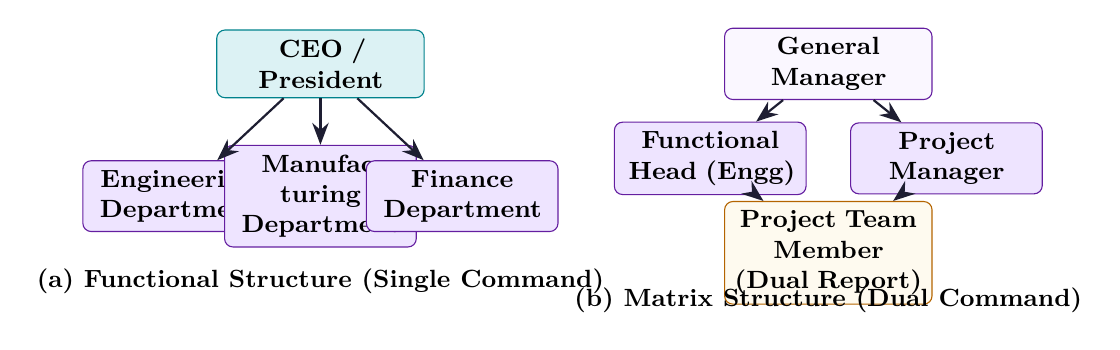
\begin{tikzpicture}[x=1.5cm, y=1.2cm]
  % Functional Structure Diagram (Left)
  \node [block] (ceo) at (1.2, 2.0) {CEO / President};
  \node [sblock] (f1) at (0.0, 0.6) {Engineering\\Department};
  \node [sblock] (f2) at (1.2, 0.6) {Manufacturing\\Department};
  \node [sblock] (f3) at (2.4, 0.6) {Finance\\Department};
  
  \draw [arrow] (ceo) -- (f1);
  \draw [arrow] (ceo) -- (f2);
  \draw [arrow] (ceo) -- (f3);
  \node at (1.2, -0.3) {\small\textbf{(a) Functional Structure (Single Command)}};

  % Matrix Structure Diagram (Right)
  \node [block, fill=hdrpurple!30, draw=mypurple] (mceo) at (5.5, 2.0) {General Manager};
  \node [sblock] (mf) at (4.5, 1.0) {Functional\\Head (Engg)};
  \node [sblock] (pm) at (6.5, 1.0) {Project\\Manager};
  \node [block, fill=hdramber!40, draw=myamber] (team) at (5.5, 0.0) {Project Team\\Member (Dual Report)};

  \draw [arrow] (mceo) -- (mf);
  \draw [arrow] (mceo) -- (pm);
  \draw [arrow] (mf) -- (team);
  \draw [arrow] (pm) -- (team);
  \node at (5.5, -0.5) {\small\textbf{(b) Matrix Structure (Dual Command)}};
\end{tikzpicture}
\end{tcolorbox}

% ===============================================================================
% 4. NATURE AND MODELS OF ORGANIZATIONAL BEHAVIOR
% ===============================================================================
\section{Nature and Scope of Organizational Behavior (OB)}

\textbf{Organizational Behavior (OB)} is an applied behavioral science field that investigates the impact of individuals, groups, and organizational structure on behavior within organizations, for the purpose of applying such knowledge toward improving organizational effectiveness.

\begin{tcolorbox}[defbox, title={Nature of Organizational Behavior}]
  OB is a \textbf{multidisciplinary field} drawing concepts from Psychology (individual level), Sociology \& Social Psychology (group level), and Anthropology \& Political Science (organization system level). It is humanistic, goal-oriented, and science-backed.
\end{tcolorbox}

\subsection{The 5 Fundamental Models of Organizational Behavior}
Organizational culture and managerial philosophy dictate the dominant OB model adopted by a firm:

\par\vspace{6pt}\noindent
\begingroup
\setlength{\tabcolsep}{2.5pt}%
\setlength{\extrarowheight}{3.5pt}%
\renewcommand{\arraystretch}{1.4}%
\footnotesize
\begin{tabularx}{\linewidth}{|>{\raggedright\arraybackslash\bfseries}p{1.9cm}|Y|Y|Y|Y|Y|}
\hline
\multicolumn{1}{|c|}{\textbf{Dimension}} & \multicolumn{1}{c|}{\textbf{Autocratic}} & \multicolumn{1}{c|}{\textbf{Custodial}} & \multicolumn{1}{c|}{\textbf{Supportive}} & \multicolumn{1}{c|}{\textbf{Collegial}} & \multicolumn{1}{c|}{\textbf{System}} \\
\hline
Basis of Model & Power / Authority & Economic resources & Leadership & Partnership & Community \\
\hline
Managerial Orientation & Authority & Money / Benefits & Support & Teamwork & Nurturing \\
\hline
Employee Orientation & Obedience & Security \& Benefit & Job performance & Responsibility & Self-discipline \\
\hline
Employee Psychological Result & Dependence on boss & Dependence on organization & Participation & Self-\allowbreak actualization & Passion \& Commitment \\
\hline
Employee Needs Met & Subsistence (Basic) & Security & Esteem & Self-\allowbreak actualization & Higher-\allowbreak order needs \\
\hline
\end{tabularx}
\endgroup

% ===============================================================================
% QUICK REVISION PAGE
% ===============================================================================
\newpage
\begin{center}
  {\large\bfseries\color{myred} Quick Revision --- Module 1}\\[3pt]
  {\small\color{mydark} Introduction to Organization \& Organizational Behavior $|$ OE-EC804C}
\end{center}
\vspace{-4pt}
\hrule
\vspace{8pt}

\begin{tcolorbox}[formulabox, title={\textbf{Key Concepts and Metrics at a Glance}}]
\renewcommand{\arraystretch}{1.35}
\begin{tabularx}{\linewidth}{>{\raggedright\arraybackslash\bfseries}p{4.5cm} X}
Organization & Social entity consciously coordinated to achieve pre-determined common goals. \\[4pt]
Formal vs Informal Org & Official hierarchical structure vs. spontaneous personal social network (grapevine). \\[4pt]
Fayol's Unity of Command & Principle stating each employee reports to one and only one direct manager. \\[4pt]
Matrix Structure & Dual-authority structure combining functional specialization with project teams. \\[4pt]
OB Field Basis & Multidisciplinary study of individual, group, and structural impact on behavior. \\[4pt]
5 OB Models & Autocratic (Power), Custodial (Security), Supportive (Leadership), Collegial (Teamwork), System (Community). \\
\end{tabularx}
\end{tcolorbox}

\begin{tcolorbox}[defbox, title={\textbf{One-Line Definitions for Exam Revision}}]
  \begin{itemize}[leftmargin=*, itemsep=2pt]
    \item \textbf{Span of Control:} The maximum number of subordinates a manager directly and effectively supervises.
    \item \textbf{Grapevine:} The informal, un official communication channel operating within an organization.
    \item \textbf{Scalar Chain:} The unbroken vertical chain of command from highest executive to lowest worker.
    \item \textbf{Organizational Structure:} The formal framework defining how job tasks are divided, grouped, and coordinated.
  \end{itemize}
\end{tcolorbox}

\begin{tcolorbox}[exambox, title={\textbf{Frequently Asked / Viva Questions}}]
\begin{enumerate}[leftmargin=*, itemsep=4pt]
  \Q{Define an Organization. What are its core components?}{An organization is a consciously coordinated social unit of two or more people working continuously toward common goals. Its core components are People, Structure, Technology, and Environment.}
  
  \Q{Differentiate between Formal and Informal Organizations.}{Formal organizations are officially created by management with rigid hierarchies and written rules. Informal organizations emerge spontaneously among employees to fulfill personal social needs.}
  
  \Q{What is Fayol's Unity of Command principle? Why is it important?}{It states that an employee should receive orders from only one manager. It prevents dual-subordination conflict, confusion, and responsibility shifting.}
  
  \Q{Explain the Matrix Organizational Structure and its major drawback.}{A matrix structure combines functional departments with project teams, creating a dual reporting line. Its main drawback is potential conflict of authority between functional and project managers.}
  
  \Q{What is Organizational Behavior (OB)?}{OB is an applied behavioral science field studying how individuals, groups, and organizational structures influence behavior, aiming to enhance organizational performance.}
  
  \Q{List the 5 primary models of Organizational Behavior.}{Autocratic (power-based), Custodial (money-based), Supportive (leadership-based), Collegial (teamwork-based), and System (community-based).}
  
  \Q{What is Span of Control? Distinguish between Tall and Flat structures.}{Span of control is the number of direct subordinates under a manager. A narrow span produces a Tall structure (many hierarchy levels); a wide span produces a Flat structure (few hierarchy levels).}
  
  \Q{How does Psychology contribute to Organizational Behavior?}{Psychology provides theories on individual behavior, learning, personality, perception, motivation, and job satisfaction.}
  
  \Q{What is the difference between Line and Staff managers?}{Line managers have direct command authority over operational tasks; Staff managers act as advisors providing specialized technical, legal, or HR guidance.}
  
  \Q{Which OB model is oriented towards meeting employee security needs?}{The Custodial model, which relies on economic resources and benefits to fulfill employee safety and financial security needs.}
\end{enumerate}
\end{tcolorbox}


% -- Module 2 -----------------------------------------------------------------
\modulestart{2}{Personality: Concept and Determinants}

\section{Personality: Concept and Determinants}

\textbf{Personality} represents the relatively stable set of psychological characteristics, behavioral patterns, and emotional tendencies that shape how an individual interacts with their environment.

\begin{tcolorbox}[defbox, title={Definition of Personality}]
  \textbf{Personality} is the dynamic organization within the individual of those psychophysical systems that determine their unique adjustments to their environment (Gordon Allport).
\end{tcolorbox}

\subsection{Determinants of Personality}
An individual's personality is shaped by four major determinants:

\begin{enumerate}[leftmargin=*, itemsep=4pt]
  \item \textbf{Heredity (Biological Factors):} Genetic traits inherited from parents (temperament, physical stature, reflexes, facial features). Twins studies show genetics accounts for nearly $50\%$ of personality variation.
  \item \textbf{Environmental Factors:} Socialization, family background, upbringing, social status, and educational experiences during early childhood.
  \item \textbf{Cultural Factors:} Cultural norms, values, beliefs, and societal expectations that dictate acceptable behavior.
  \item \textbf{Situational Factors:} Specific events, crises, or work situations that constrain or draw out specific personality dimensions.
\end{enumerate}

\subsection{Personality Development: Theories and Stages}
Personality development refers to the process by which an individual's unique behavioral patterns and psychological structures evolve over time:

\begin{enumerate}[leftmargin=*, itemsep=4pt]
  \item \textbf{Freud's Psychoanalytic Theory:} Personality consists of three interacting structural systems:
    \begin{itemize}[leftmargin=*, noitemsep]
      \item \textit{Id:} Unconscious, primitive drive operating on the pleasure principle.
      \item \textit{Ego:} Realistic, conscious executive operating on the reality principle.
      \item \textit{Superego:} Moral conscience representing societal norms and ethical ideals.
    \end{itemize}
  \item \textbf{Erikson's 8 Psychosocial Stages:} Personality evolves through 8 life stages characterized by specific psychosocial crises (e.g., Trust vs. Mistrust, Identity vs. Role Confusion, Industry vs. Inferiority).
  \item \textbf{Argyris' Immaturity-Maturity Continuum:} Chris Argyris proposed that individuals naturally progress along a continuum from infant \textbf{immaturity} (passive, dependent, short-term perspective) to adult \textbf{maturity} (active, independent, long-term perspective, self-awareness).
\end{enumerate}

% ===============================================================================
% 2. PERSONALITY THEORIES AND APPLICATIONS IN OB
% ===============================================================================
\section{Personality Theories and Applications in OB}

\subsection{The Big Five Personality Traits Model (OCEAN)}
The \textbf{Big Five Model} is the most widely validated framework for assessing personality traits in business settings:

\par\vspace{6pt}\noindent
\begingroup
\setlength{\tabcolsep}{5pt}%
\setlength{\extrarowheight}{3pt}%
\renewcommand{\arraystretch}{1.35}%
\begin{tabularx}{\linewidth}{|>{\raggedright\arraybackslash\bfseries}p{3.2cm}|Y|Y|}
\hline
\multicolumn{1}{|c|}{\textbf{Trait}} & \multicolumn{1}{c|}{\textbf{High Score Characteristics}} & \multicolumn{1}{c|}{\textbf{Organizational Impact}} \\
\hline
Openness to Experience & Creative, curious, imaginative, insightful, flexible. & Adapts quickly to organizational change \& innovation. \\
\hline
Conscientiousness & Organized, dependable, thorough, disciplined, goal-driven. & Single strongest predictor of overall job performance. \\
\hline
Extraversion & Sociable, assertive, energetic, outgoing, talkative. & Performs exceptionally in sales, leadership, \& networking. \\
\hline
Agreeableness & Cooperative, trusting, empathetic, warm, helpful. & Excels in teamwork, customer service, \& conflict resolution. \\
\hline
Emotional Stability (vs. Neuroticism) & Calm, self-confident, secure, stress-resilient. & High job satisfaction; low occupational burnout. \\
\hline
\end{tabularx}
\endgroup

\subsection{Major Personality Attributes Influencing OB}
\begin{itemize}[leftmargin=*, itemsep=4pt]
  \item \textbf{Locus of Control:} Belief about who controls destiny.
    \begin{itemize}[leftmargin=*, noitemsep]
      \item \textit{Internals:} Believe outcomes stem from their own effort. Higher job satisfaction \& performance.
      \item \textit{Externals:} Believe outcomes are driven by luck, fate, or external power. Higher stress.
    \end{itemize}
  \item \textbf{Machiavellianism (High-Mach):} Pragmatic, emotionally distant, and believes "the end justifies the means". Excels in high-stakes negotiations.
  \item \textbf{Type A vs. Type B Personality:}
    \begin{itemize}[leftmargin=*, noitemsep]
      \item \textit{Type A:} Impatient, competitive, time-conscious, aggressive. Prone to work stress.
      \item \textit{Type B:} Relaxed, patient, steady, non-competitive. Better long-term strategic thinkers.
    \end{itemize}
  \item \textbf{Self-Monitoring:} Ability to adjust behavior to external situational factors. High self-monitors are adept at political maneuvering.
\end{itemize}

% ===============================================================================
% 3. MOTIVATION CONCEPTS AND THEORIES
% ===============================================================================
\section{Motivation: Concepts and Theories}

\textbf{Motivation} is the psychological process that initiates, directs, and sustains goal-oriented human behavior.

\begin{tcolorbox}[defbox, title={Definition of Motivation}]
  \textbf{Motivation} is the willingness to exert high levels of effort toward organizational goals, conditioned by the effort's ability to satisfy some individual need (Robbins).
\end{tcolorbox}

\subsection{The Motivation-Behavior Process}

\begin{tcolorbox}[tikzbox, title={The 6-Stage Motivation-Behavior Process}]
\centering
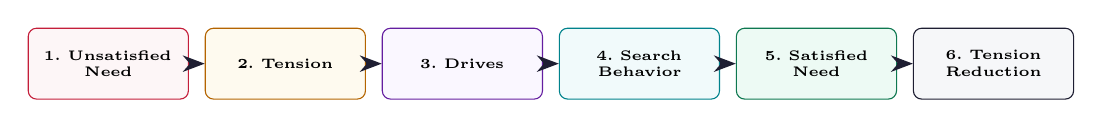
\begin{tikzpicture}[sblock/.style={rectangle, draw=mydark, fill=hdrteal!30, rounded corners=3pt, align=center, font=\tiny\bfseries, minimum height=0.9cm, text width=1.8cm}, node distance=0.2cm, auto]
  \node [sblock, fill=hdrred!40, draw=myred] (n) {1. Unsatisfied\\Need};
  \node [sblock, right=0.2cm of n, fill=hdramber!40, draw=myamber] (t) {2. Tension};
  \node [sblock, right=0.2cm of t, fill=hdrpurple!30, draw=mypurple] (d) {3. Drives};
  \node [sblock, right=0.2cm of d, fill=hdrteal!40, draw=myteal] (s) {4. Search\\Behavior};
  \node [sblock, right=0.2cm of s, fill=hdrgreen!50, draw=mygreen] (sat) {5. Satisfied\\Need};
  \node [sblock, right=0.2cm of sat, fill=mygray, draw=mydark] (r) {6. Tension\\Reduction};

  \draw [arrow] (n) -- (t);
  \draw [arrow] (t) -- (d);
  \draw [arrow] (d) -- (s);
  \draw [arrow] (s) -- (sat);
  \draw [arrow] (sat) -- (r);
\end{tikzpicture}
\end{tcolorbox}

\subsection{Maslow's Hierarchy of Needs Theory}
Abraham Maslow posited that human needs are arranged in a 5-level hierarchy. Individuals satisfy lower-order needs before progressing to higher-order needs:

\begin{tcolorbox}[tikzbox, title={Maslow's Hierarchy of Needs Pyramid}]
\centering
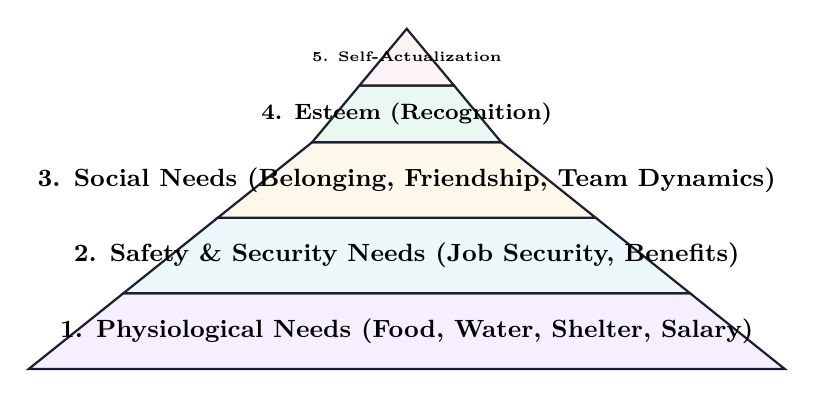
\begin{tikzpicture}[x=1.2cm, y=0.8cm]
  % Pyramid Slices
  \draw[line, fill=hdrpurple!60] (-4,0) -- (4,0) -- (3,1.2) -- (-3,1.2) -- cycle;
  \node at (0,0.6) {\small\textbf{1. Physiological Needs (Food, Water, Shelter, Salary)}};
  
  \draw[line, fill=hdrteal!50] (-3,1.2) -- (3,1.2) -- (2,2.4) -- (-2,2.4) -- cycle;
  \node at (0,1.8) {\small\textbf{2. Safety \& Security Needs (Job Security, Benefits)}};
  
  \draw[line, fill=hdramber!50] (-2,2.4) -- (2,2.4) -- (1,3.6) -- (-1,3.6) -- cycle;
  \node at (0,3.0) {\small\textbf{3. Social Needs (Belonging, Friendship, Team Dynamics)}};
  
  \draw[line, fill=hdrgreen!60] (-1,3.6) -- (1,3.6) -- (0.5,4.5) -- (-0.5,4.5) -- cycle;
  \node at (0,4.05) {\footnotesize\textbf{4. Esteem (Recognition)}};
  
  \draw[line, fill=hdrred!50] (-0.5,4.5) -- (0.5,4.5) -- (0,5.4) -- cycle;
  \node at (0,4.95) {\tiny\textbf{5. Self-Actualization}};
\end{tikzpicture}
\end{tcolorbox}

\subsection{Herzberg's Two-Factor (Hygiene-Motivator) Theory}
Frederick Herzberg proposed that job satisfaction and job dissatisfaction are driven by two independent sets of factors:

\par\vspace{6pt}\noindent
\begingroup
\setlength{\tabcolsep}{5pt}%
\setlength{\extrarowheight}{3pt}%
\renewcommand{\arraystretch}{1.35}%
\begin{tabularx}{\linewidth}{|>{\raggedright\arraybackslash\bfseries}p{3.5cm}|Y|Y|}
\hline
\multicolumn{1}{|c|}{\textbf{Dimension}} & \multicolumn{1}{c|}{\textbf{Hygiene Factors (Extrinsic)}} & \multicolumn{1}{c|}{\textbf{Motivators (Intrinsic)}} \\
\hline
Primary Impact & Prevents job dissatisfaction (does NOT create motivation). & Generates high job satisfaction \& intrinsic motivation. \\
\hline
Factors & Salary, company policies, working conditions, job security, supervision. & Achievement, recognition, responsibility, advancement, work itself. \\
\hline
Absence Result & Severe job dissatisfaction. & Neutral state (no satisfaction, but no dissatisfaction). \\
\hline
\end{tabularx}
\endgroup

\subsection{McGregor's Theory X and Theory Y}
Douglas McGregor formulated two contrasting views of human workforce motivation:

\par\vspace{6pt}\noindent
\begingroup
\setlength{\tabcolsep}{5pt}%
\setlength{\extrarowheight}{3pt}%
\renewcommand{\arraystretch}{1.35}%
\begin{tabularx}{\linewidth}{|>{\raggedright\arraybackslash\bfseries}p{3.5cm}|Y|Y|}
\hline
\multicolumn{1}{|c|}{\textbf{Assumption Area}} & \multicolumn{1}{c|}{\textbf{Theory X (Authoritarian View)}} & \multicolumn{1}{c|}{\textbf{Theory Y (Participative View)}} \\
\hline
Attitude Toward Work & Inherently dislike work and avoid it whenever possible. & View work as natural as play or rest. \\
\hline
Ambition \& Responsibility & Lack ambition, avoid responsibility, seek direction. & Exercise self-direction, seek responsibility. \\
\hline
Managerial Strategy & Strict control, coercion, punishment, close supervision. & Empowerment, delegation, participative decision-making. \\
\hline
Primary Motivator & Lower-order physiological \& safety needs. & Higher-order esteem \& self-actualization needs. \\
\hline
\end{tabularx}
\endgroup

% ===============================================================================
% 4. MOTIVATIONAL SYSTEMS AND INDIAN ORGANIZATIONAL CONTEXT
% ===============================================================================
\section{Elements of Sound Motivational System \& Indian Context}

\subsection{Elements of a Sound Motivational System}
A comprehensive managerial motivation strategy integrates financial and non-financial rewards:
\begin{itemize}[leftmargin=*, itemsep=4pt]
  \item \textbf{Fair \& Competitive Compensation:} Merit-based pay, profit sharing, and performance bonuses.
  \item \textbf{Job Enrichment:} Expanding job content vertically by giving greater autonomy, responsibility, and decision-making power.
  \item \textbf{Job Enlargement:} Expanding job content horizontally by adding a wider variety of similar tasks to eliminate monotony.
  \item \textbf{Employee Recognition Programs:} Awards, promotions, and public praise.
\end{itemize}

\subsection{Motivation in Indian Organizations}
Motivation strategies in Indian corporate environments account for cultural nuances (collectivism, respect for hierarchy, family orientation):
\begin{itemize}[leftmargin=*, itemsep=3pt]
  \item High value placed on \textbf{job security} and institutional stability.
  \item Paternalistic leadership style offering personal care alongside professional direction.
  \item Growing shift toward performance-linked incentives (PLI) and stock options (ESOPs) in tech startups and IT sectors.
\end{itemize}

% ===============================================================================
% QUICK REVISION PAGE
% ===============================================================================
\newpage
\begin{center}
  {\large\bfseries\color{myred} Quick Revision --- Module 2}\\[3pt]
  {\small\color{mydark} Personality and Motivation $|$ OE-EC804C}
\end{center}
\vspace{-4pt}
\hrule
\vspace{8pt}

\begin{tcolorbox}[formulabox, title={\textbf{Key Concepts and Metrics at a Glance}}]
\renewcommand{\arraystretch}{1.35}
\begin{tabularx}{\linewidth}{>{\raggedright\arraybackslash\bfseries}p{4.5cm} X}
Big Five OCEAN & Openness, Conscientiousness, Extraversion, Agreeableness, Neuroticism. \\[4pt]
Locus of Control & Internal (effort controls outcomes) vs. External (luck/fate controls outcomes). \\[4pt]
Maslow's Hierarchy & 5-stage needs pyramid: Physiological $\to$ Safety $\to$ Social $\to$ Esteem $\to$ Self-Actualization. \\[4pt]
Herzberg Two-Factor & Hygiene factors (salary/policy prevent dissatisfaction) vs. Motivators (responsibility/recognition build satisfaction). \\[4pt]
Theory X vs Theory Y & Lazy, coercive workforce view (Theory X) vs. Self-motivated, creative workforce view (Theory Y). \\
\end{tabularx}
\end{tcolorbox}

\begin{tcolorbox}[defbox, title={\textbf{One-Line Definitions for Exam Revision}}]
  \begin{itemize}[leftmargin=*, itemsep=2pt]
    \item \textbf{Conscientiousness:} Big Five trait reflecting organization, dependability, and goal discipline.
    \item \textbf{Machiavellianism:} Personality attribute characterized by emotional detachment and belief that ends justify means.
    \item \textbf{Job Enrichment:} Vertical expansion of job duties to increase employee autonomy and responsibility.
    \item \textbf{Hygiene Factors:} Extrinsic job factors whose presence prevents dissatisfaction but does not motivate.
  \end{itemize}
\end{tcolorbox}

\begin{tcolorbox}[exambox, title={\textbf{Frequently Asked / Viva Questions}}]
\begin{enumerate}[leftmargin=*, itemsep=4pt]
  \Q{Define Personality. What are its four main determinants?}{Personality is the dynamic organization of psychophysical systems determining an individual's unique adjustment to environment. Determinants: Heredity, Environment, Culture, and Situation.}
  
  \Q{List the Big Five personality traits (OCEAN). Which trait best predicts job performance?}{Openness, Conscientiousness, Extraversion, Agreeableness, and Neuroticism (Emotional Stability). Conscientiousness is the single best predictor of overall job performance.}
  
  \Q{Differentiate between Internal and External Locus of Control.}{Internals believe their own efforts determine success/failure; Externals believe outcomes are dictated by outside forces like luck, fate, or powerful people.}
  
  \Q{Compare Type A and Type B personalities.}{Type A individuals are impatient, competitive, aggressive, and time-driven; Type B individuals are relaxed, steady, patient, and less prone to stress.}
  
  \Q{Explain Maslow's Need Hierarchy Theory.}{Maslow proposed human needs follow a 5-tier pyramid: Physiological, Safety, Social, Esteem, and Self-Actualization. Individuals must fulfill lower-level needs before higher-level needs motivate them.}
  
  \Q{What are Hygiene Factors according to Herzberg? Give examples.}{Hygiene factors are extrinsic job elements (salary, company policy, working conditions) that prevent job dissatisfaction when present, but do not create positive motivation.}
  
  \Q{Contrast McGregor's Theory X and Theory Y.}{Theory X assumes workers are inherently lazy, dislike responsibility, and require coercion; Theory Y assumes workers are self-motivated, creative, and seek responsibility.}
  
  \Q{What is the difference between Job Enlargement and Job Enrichment?}{Job Enlargement expands work horizontally by adding similar tasks; Job Enrichment expands work vertically by adding autonomy, planning, and control.}
  
  \Q{Define Machiavellianism in an organizational context.}{It is a personality trait where an individual is pragmatic, maintains emotional distance, and manipulates situations believing the end justifies the means.}
  
  \Q{What factors influence employee motivation in Indian organizations?}{Job security, family-oriented benefits, respect for hierarchy, paternalistic leadership, and performance-linked incentives.}
\end{enumerate}
\end{tcolorbox}


% -- Module 3 -----------------------------------------------------------------
\modulestart{3}{Leadership: Concepts and Theories}

\section{Leadership: Concepts and Theories}

\textbf{Leadership} is the process of influencing, motivating, and directing followers toward the achievement of organizational vision and objectives.

\begin{tcolorbox}[defbox, title={Definition of Leadership}]
  \textbf{Leadership} is the ability to influence a group toward the achievement of a vision or set of goals (Stephen P. Robbins).
\end{tcolorbox}

\subsection{Distinction: Manager vs. Leader}

\par\vspace{6pt}\noindent
\begingroup
\setlength{\tabcolsep}{5pt}%
\setlength{\extrarowheight}{3pt}%
\renewcommand{\arraystretch}{1.35}%
\begin{tabularx}{\linewidth}{|>{\raggedright\arraybackslash\bfseries}p{3.2cm}|Y|Y|}
\hline
\multicolumn{1}{|c|}{\textbf{Dimension}} & \multicolumn{1}{c|}{\textbf{Manager}} & \multicolumn{1}{c|}{\textbf{Leader}} \\
\hline
Source of Power & Formal positional authority granted by organization. & Personal influence, charisma, and follower trust. \\
\hline
Primary Orientation & Planning, budgeting, organizing, controlling, stability. & Setting vision, aligning people, inspiring, driving change. \\
\hline
Focus & Systems, structures, processes, efficiency. & People, relationships, values, culture. \\
\hline
Time Horizon & Short-term to medium-term operational targets. & Long-term strategic vision. \\
\hline
\end{tabularx}
\endgroup

\subsection{Major Theories of Leadership}
\begin{enumerate}[leftmargin=*, itemsep=5pt]
  \item \textbf{Trait Theory (Great Man Theory):} Assumes leaders possess inherent physical, intellectual, and personality traits (intelligence, self-confidence, integrity, drive, emotional maturity).
  \item \textbf{Behavioral Theories:} Focuses on specific observable behaviors rather than traits.
    \begin{itemize}[leftmargin=*, noitemsep]
      \item \textit{Ohio State Studies:} Identified two dimensions --- \textbf{Initiating Structure} (task-oriented) and \textbf{Consideration} (people-oriented).
      \item \textit{Michigan Studies:} Identified \textbf{Production-Oriented} vs. \textbf{Employee-Oriented} leadership behaviors.
      \item \textit{Blake-Mouton Managerial Grid:} 9x9 matrix plotting \textbf{Concern for Production} vs. \textbf{Concern for People}.
    \end{itemize}
  \item \textbf{Contingency / Situational Theories:} Effective leadership depends on matching leadership style to situational variables (Fiedler's Contingency Model, Hersey-Blanchard Situational Leadership).
\end{enumerate}

\subsection{Blake-Mouton Managerial Grid Styles}
\begin{itemize}[leftmargin=*, itemsep=3pt]
  \item \textbf{Impoverished Management (1,1):} Low production, low people concern (minimal effort).
  \item \textbf{Country Club Management (1,9):} High people concern, low production concern (friendly atmosphere, low output).
  \item \textbf{Task / Authority Management (9,1):} High production concern, low people concern (autocratic efficiency).
  \item \textbf{Middle-of-the-Road Management (5,5):} Balanced, adequate performance.
  \item \textbf{Team Management (9,9):} High production, high people concern (\textbf{Optimal style}).
\end{itemize}

% ===============================================================================
% 2. LEADERSHIP STYLES AND INDIAN CORPORATE CONTEXT
% ===============================================================================
\section{Leadership Styles and Indian Corporate Context}

\subsection{Classical Leadership Styles}
\begin{itemize}[leftmargin=*, itemsep=4pt]
  \item \textbf{Autocratic (Authoritarian):} Centralized decision-making; top-down commands without subordinate participation. Effective in emergency/crisis situations.
  \item \textbf{Democratic (Participative):} Decentralized decision-making; subordinate participation encouraged. Fosters commitment and high morale.
  \item \textbf{Laissez-Faire (Free-Rein):} Complete freedom granted to subordinates; leader acts as passive resource provider. Effective only with highly skilled experts.
\end{itemize}

\subsection{Transformational vs. Transactional Leadership}

\par\vspace{6pt}\noindent
\begingroup
\setlength{\tabcolsep}{5pt}%
\setlength{\extrarowheight}{3pt}%
\renewcommand{\arraystretch}{1.35}%
\begin{tabularx}{\linewidth}{|>{\raggedright\arraybackslash\bfseries}p{3.2cm}|Y|Y|}
\hline
\multicolumn{1}{|c|}{\textbf{Feature}} & \multicolumn{1}{c|}{\textbf{Transactional Leadership}} & \multicolumn{1}{c|}{\textbf{Transformational Leadership}} \\
\hline
Core Mechanism & Exchange process (rewards for compliance, punishment for failure). & Inspires followers to transcend self-interest for organizational vision. \\
\hline
Focus & Maintaining current operations \& status quo. & Driving organizational change, innovation, \& renewal. \\
\hline
Key Components & Contingent Reward, Management by Exception (Active/Passive). & Idealized Influence, Inspirational Motivation, Intellectual Stimulation. \\
\hline
Impact & Expected standard performance. & Performance beyond expectations. \\
\hline
\end{tabularx}
\endgroup

\subsection{Leadership in Indian Organizations}
Indian corporate leadership is uniquely characterized by:
\begin{itemize}[leftmargin=*, itemsep=3pt]
  \item \textbf{Paternalistic Approach:} Combining firm authority with nurturance, family-like care, and guidance.
  \item High respect for age, seniority, and organizational hierarchy.
  \item Rapid transition toward participative, transformational leadership in technology and global enterprise sectors.
\end{itemize}

% ===============================================================================
% 3. GROUP DYNAMICS AND STAGES OF GROUP DEVELOPMENT
% ===============================================================================
\section{Group Dynamics and Stages of Development}

A \textbf{Group} consists of two or more interacting individuals who come together to achieve particular objectives.

\begin{tcolorbox}[defbox, title={Concept of Group Dynamics}]
  \textbf{Group Dynamics} refers to the complex social forces, interactions, processes, and behavioral patterns operating within and between human groups.
\end{tcolorbox}

\subsection{Types of Groups}
\begin{itemize}[leftmargin=*, itemsep=3pt]
  \item \textbf{Formal Groups:} Created by management (Command Groups, Task Forces, Committees).
  \item \textbf{Informal Groups:} Spontaneously formed by members (Interest Groups, Friendship Groups).
\end{itemize}

\subsection{Tuckman's 5 Stages of Group Development}
Groups evolve through five sequential stages during their lifecycle:

\begin{tcolorbox}[tikzbox, title={Tuckman's 5 Stages of Group Development}]
\centering
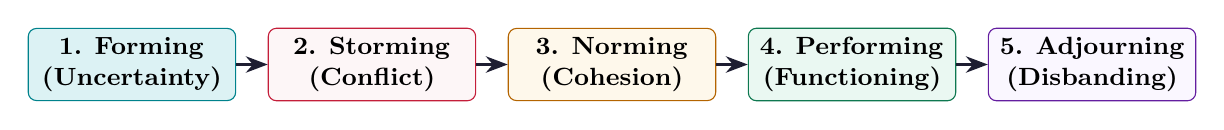
\begin{tikzpicture}[node distance=0.5cm, auto]
  \node [block] (f) {1. Forming\\(Uncertainty)};
  \node [block, right=0.4cm of f, fill=hdrred!40, draw=myred] (s) {2. Storming\\(Conflict)};
  \node [block, right=0.4cm of s, fill=hdramber!50, draw=myamber] (n) {3. Norming\\(Cohesion)};
  \node [block, right=0.4cm of n, fill=hdrgreen!60, draw=mygreen] (p) {4. Performing\\(Functioning)};
  \node [block, right=0.4cm of p, fill=hdrpurple!30, draw=mypurple] (a) {5. Adjourning\\(Disbanding)};

  \draw [arrow] (f) -- (s);
  \draw [arrow] (s) -- (n);
  \draw [arrow] (n) -- (p);
  \draw [arrow] (p) -- (a);
\end{tikzpicture}
\end{tcolorbox}

\begin{enumerate}[leftmargin=*, itemsep=3pt]
  \item \textbf{Forming:} Initial orientation, high uncertainty, testing boundaries and group purpose.
  \item \textbf{Storming:} Intra-group conflict, power struggles, resistance to group constraints.
  \item \textbf{Norming:} Close relationships develop, strong group identity, consensus on norms.
  \item \textbf{Performing:} Group structure becomes fully functional and accepted; focus shifts to task execution.
  \item \textbf{Adjourning:} Disbanding after goal completion (for temporary task groups).
\end{enumerate}

\subsection{Group Behavior: Norms, Cohesiveness, and Roles}
Understanding group behavior requires analyzing three fundamental properties:
\begin{enumerate}[leftmargin=*, itemsep=4pt]
  \item \textbf{Group Norms:} Acceptable standards of behavior shared by group members (performance norms, appearance norms, social arrangement norms).
  \item \textbf{Group Cohesiveness:} The degree to which group members are attracted to each other and motivated to stay in the group.
    \begin{itemize}[leftmargin=*, noitemsep]
      \item \textit{High Cohesiveness + High Performance Norms:} Results in \textbf{highest productivity}.
      \item \textit{High Cohesiveness + Low Performance Norms:} Results in \textbf{low productivity} (group restricts output).
    \end{itemize}
  \item \textbf{Group Conformity \& Asch Effect:} The tendency for members to align their perceptions, opinions, and behaviors with group norms due to social pressure.
\end{enumerate}

% ===============================================================================
% 4. GROUP DECISION MAKING TECHNIQUES AND MERITS/DEMERITS
% ===============================================================================
\section{Group Decision Making: Techniques, Merits, and Demerits}

\subsection{Techniques to Improve Group Decision Making}
\begin{enumerate}[leftmargin=*, itemsep=4pt]
  \item \textbf{Brainstorming:} Idea-generation process encouraging free thinking without criticism.
  \item \textbf{Nominal Group Technique (NGT):} Structured meeting where members write ideas independently before silent voting to prioritize solutions.
  \item \textbf{Delphi Technique:} Systematic decision process collecting anonymous expert opinions via sequential questionnaires without physical meeting.
  \item \textbf{Electronic Meetings:} Combining NGT with computer networking for anonymous real-time voting.
\end{enumerate}

\subsection{Merits and Demerits of Group Decision Making}

\par\vspace{6pt}\noindent
\begingroup
\setlength{\tabcolsep}{5pt}%
\setlength{\extrarowheight}{3pt}%
\renewcommand{\arraystretch}{1.35}%
\begin{tabularx}{\linewidth}{|Y|Y|}
\hline
\multicolumn{1}{|c|}{\textbf{Merits / Advantages}} & \multicolumn{1}{c|}{\textbf{Demerits / Disadvantages}} \\
\hline
\textbf{Complete Information \& Knowledge:} Aggregates diverse expertise, skills, and perspectives. & \textbf{Time-Consuming:} Takes longer to schedule, discuss, and reach consensus compared to individual decisions. \\
\hline
\textbf{Increased Acceptance:} Participants feel ownership, leading to smoother implementation. & \textbf{Groupthink:} Conformity pressure suppresses critical, divergent thinking. \\
\hline
\textbf{Diversity of Views:} Generates more alternatives and creative solutions. & \textbf{Domination by Few:} Vocal or influential members can dominate discussions. \\
\hline
\textbf{Legitimacy:} Democratic consensus decisions are perceived as more legitimate. & \textbf{Ambiguous Responsibility:} Shared accountability dilutes individual responsibility. \\
\hline
\end{tabularx}
\endgroup

% ===============================================================================
% QUICK REVISION PAGE
% ===============================================================================
\newpage
\begin{center}
  {\large\bfseries\color{myred} Quick Revision --- Module 3}\\[3pt]
  {\small\color{mydark} Leadership and Group Dynamics $|$ OE-EC804C}
\end{center}
\vspace{-4pt}
\hrule
\vspace{8pt}

\begin{tcolorbox}[formulabox, title={\textbf{Key Concepts and Metrics at a Glance}}]
\renewcommand{\arraystretch}{1.35}
\begin{tabularx}{\linewidth}{>{\raggedright\arraybackslash\bfseries}p{4.5cm} X}
Manager vs Leader & Positional authority/control (Manager) vs. Personal influence/vision (Leader). \\[4pt]
Managerial Grid & Blake-Mouton 9x9 grid (Optimal style: 9,9 Team Management). \\[4pt]
Tuckman's 5 Stages & Forming $\to$ Storming $\to$ Norming $\to$ Performing $\to$ Adjourning. \\[4pt]
Groupthink & Phenomenon where pressure for conformity overrides critical appraisal of alternatives. \\[4pt]
Delphi Technique & Decision-making technique using anonymous expert questionnaires. \\
\end{tabularx}
\end{tcolorbox}

\begin{tcolorbox}[defbox, title={\textbf{One-Line Definitions for Exam Revision}}]
  \begin{itemize}[leftmargin=*, itemsep=2pt]
    \item \textbf{Transformational Leadership:} Style inspiring followers to transcend self-interest for strategic organizational vision.
    \item \textbf{Group Dynamics:} The social interactions and behavioral forces operating within human groups.
    \item \textbf{Nominal Group Technique:} Structured group decision method restricting discussion during initial idea generation.
    \item \textbf{Groupthink:} Deterioration of mental efficiency and moral judgment resulting from in-group pressures.
  \end{itemize}
\end{tcolorbox}

\begin{tcolorbox}[exambox, title={\textbf{Frequently Asked / Viva Questions}}]
\begin{enumerate}[leftmargin=*, itemsep=4pt]
  \Q{Define Leadership. How does a Leader differ from a Manager?}{Leadership is the ability to influence a group toward achieving a vision. Managers rely on formal authority for stability; Leaders rely on personal influence to drive change.}
  
  \Q{Explain Blake-Mouton's Managerial Grid. Which position represents optimal leadership?}{The grid plots Concern for Production vs. Concern for People on a 9x9 scale. Position (9,9) Team Management is the optimal style.}
  
  \Q{Differentiate between Transactional and Transformational Leadership.}{Transactional leadership relies on contingent exchanges and rewards; Transformational leadership inspires followers to innovate and achieve visionary goals.}
  
  \Q{Trace Tuckman's 5 stages of group development.}{Forming (orientation) $\to$ Storming (conflict) $\to$ Norming (cohesion) $\to$ Performing (functioning) $\to$ Adjourning (disbanding).}
  
  \Q{What is Group Dynamics?}{The social forces, interactions, processes, and behavioral patterns operating within and between human groups.}
  
  \Q{What is Groupthink? How can it be prevented?}{Groupthink is the pressure for conformity suppressing critical dissent. It can be prevented by assigning a devil's advocate and encouraging open feedback.}
  
  \Q{Explain the Delphi Technique of decision making.}{A systematic decision method collecting anonymous opinions from distributed experts via sequential questionnaires without physical meetings.}
  
  \Q{What are the major advantages of group decision making over individual decision making?}{Groups provide more complete information, diverse perspectives, creative alternatives, and higher implementation acceptance.}
  
  \Q{What is a Laissez-Faire leadership style? When is it effective?}{A free-rein style granting complete operational freedom to subordinates. Effective only with highly expert, self-motivated professionals.}
  
  \Q{Describe the characteristic style of leadership in Indian corporate organizations.}{Paternalistic leadership, which combines firm administrative authority with family-like personal care and nurturance.}
\end{enumerate}
\end{tcolorbox}


% -- Module 4 -----------------------------------------------------------------
\modulestart{4}{Meaning and Nature of Organizational Change}

\section{Meaning and Nature of Organizational Change}

\textbf{Organizational Change} refers to the alteration of organizational structures, operational processes, corporate culture, technologies, or strategic goals in response to internal or external environmental shifts.

\begin{tcolorbox}[defbox, title={Definition of Organizational Change}]
  \textbf{Organizational Change} is any alteration that occurs in the total organization environment (Keith Davis).
\end{tcolorbox}

\subsection{Nature of Change}
\begin{itemize}[leftmargin=*, itemsep=3pt]
  \item \textbf{Pervasive \& Continuous:} Change is an ongoing reality in corporate life.
  \item \textbf{Systemic:} A change in one department impacts all interconnected sub-systems.
  \item \textbf{Reactive vs. Proactive Change:}
    \begin{itemize}[leftmargin=*, noitemsep]
      \item \textit{Reactive Change:} Triggered by immediate crisis or market pressure.
      \item \textit{Proactive Change:} Anticipatory changes initiated to exploit future opportunities.
    \end{itemize}
\end{itemize}

\subsection{Factors Driving Organizational Change}

\par\vspace{6pt}\noindent
\begingroup
\setlength{\tabcolsep}{5pt}%
\setlength{\extrarowheight}{3pt}%
\renewcommand{\arraystretch}{1.35}%
\begin{tabularx}{\linewidth}{|>{\raggedright\arraybackslash\bfseries}p{3.5cm}|Y|Y|}
\hline
\multicolumn{1}{|c|}{\textbf{Force Category}} & \multicolumn{1}{c|}{\textbf{Driving Factors}} & \multicolumn{1}{c|}{\textbf{Examples}} \\
\hline
External Forces & Globalization, market competition, technological disruption, economic shifts, regulatory changes. & Transition to cloud computing, AI automation, regulatory ESG compliance. \\
\hline
Internal Forces & Leadership shifts, strategic realignments, operational bottlenecks, low employee morale. & Mergers, new CEO vision, enterprise resource planning (ERP) rollout. \\
\hline
\end{tabularx}
\endgroup

% ===============================================================================
% 2. RESISTANCE TO CHANGE AND OVERCOMING STRATEGIES
% ===============================================================================
\section{Resistance to Change and Overcoming Strategies}

\textbf{Resistance to Change} is human or structural opposition to alterations in established routines, habits, or power balances.

\subsection{Factors Causing Resistance}
\begin{enumerate}[leftmargin=*, itemsep=4pt]
  \item \textbf{Individual Sources of Resistance:}
    \begin{itemize}[leftmargin=*, noitemsep]
      \item \textit{Fear of the Unknown:} Anxiety over new skill requirements or job security.
      \item \textit{Habit:} Preference for familiar operational routines.
      \item \textit{Economic Insecurity:} Concern over potential salary cuts or demotion.
      \item \textit{Selective Perception:} Interpreting change information selectively.
    \end{itemize}
  \item \textbf{Organizational Sources of Resistance:}
    \begin{itemize}[leftmargin=*, noitemsep]
      \item \textit{Structural Inertia:} Rigid organizational structures designed for stability.
      \item \textit{Threat to Expertise \& Power:} Shifts threatening specialized group influence.
    \end{itemize}
\end{enumerate}

\subsection{Lewin's 3-Step Change Model}
Kurt Lewin proposed that successful organizational change follows three sequential steps:

\begin{tcolorbox}[tikzbox, title={Lewin's 3-Step Change Model}]
\centering
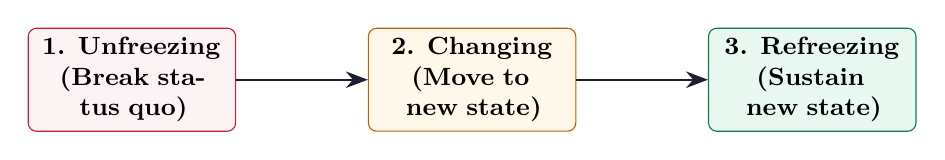
\begin{tikzpicture}[x=1.8cm, y=1.0cm]
  \node [block, fill=hdrred!50, draw=myred] (u) at (0,0) {1. Unfreezing\\(Break status quo)};
  \node [block, fill=hdramber!50, draw=myamber] (c) at (2.4,0) {2. Changing\\(Move to new state)};
  \node [block, fill=hdrgreen!60, draw=mygreen] (r) at (4.8,0) {3. Refreezing\\(Sustain new state)};

  \draw [arrow] (u) -- (c);
  \draw [arrow] (c) -- (r);
\end{tikzpicture}
\end{tcolorbox}

\begin{enumerate}[leftmargin=*, itemsep=3pt]
  \item \textbf{Unfreezing:} Disrupting the existing equilibrium by demonstrating the urgency of change and weakening driving forces of resistance.
  \item \textbf{Changing (Moving):} Implementing new processes, technology, structures, or behaviors.
  \item \textbf{Refreezing:} Institutionalizing the new state by reinforcing positive behaviors through rewards, culture, and policies.
\end{enumerate}

\subsection{Kotter's 8-Step Leading Change Model}
John Kotter proposed an 8-stage strategic framework for executing successful organizational transformations:
\begin{enumerate}[leftmargin=*, itemsep=3pt]
  \item \textbf{Establish Urgency:} Highlight market realities and financial threats to motivate change.
  \item \textbf{Form a Guiding Coalition:} Assemble a powerful team with position power and expertise to lead change.
  \item \textbf{Create a Strategic Vision:} Develop a clear vision and strategic initiatives to direct transformation.
  \item \textbf{Communicate the Vision:} Use all internal channels to communicate the vision and strategy.
  \item \textbf{Empower Broad-Based Action:} Remove structural barriers and revise systems that undermine change.
  \item \textbf{Generate Short-Term Wins:} Plan for visible, unambiguous performance improvements.
  \item \textbf{Sustain Acceleration:} Consolidate gains and produce more change.
  \item \textbf{Institute Change:} Anchor new behaviors in corporate culture and succession planning.
\end{enumerate}

\subsection{Strategies for Overcoming Resistance}
\begin{itemize}[leftmargin=*, itemsep=3pt]
  \item \textbf{Education \& Communication:} Informing employees about change logic to reduce misinformation.
  \item \textbf{Participation \& Involvement:} Involving employees in decision-making to build ownership.
  \item \textbf{Facilitation \& Support:} Providing retraining, counseling, and stress management.
  \item \textbf{Negotiation \& Agreement:} Offering incentives to powerful resistant groups.
\end{itemize}

% ===============================================================================
% 3. ORGANIZATIONAL DEVELOPMENT (OD)
% ===============================================================================
\section{Organizational Development (OD): Concept, Process, and Interventions}

\begin{tcolorbox}[defbox, title={Definition of Organizational Development (OD)}]
  \textbf{Organizational Development (OD)} is a systematic, long-term, top-management-supported effort to improve an organization's vision, empowerment, learning, and problem-solving processes through organizational culture management (Wendell French).
\end{tcolorbox}

\subsection{Core Objectives of OD}
\begin{itemize}[leftmargin=*, itemsep=3pt]
  \item Build high organizational trust, openness, and collaborative problem-solving capacity.
  \item Align organizational structure and culture with technological and strategic demands.
  \item Enhance employee satisfaction, motivation, and personal growth.
\end{itemize}

\subsection{The 4-Stage OD Process}

\begin{tcolorbox}[tikzbox, title={The 4-Stage OD Process}]
\centering
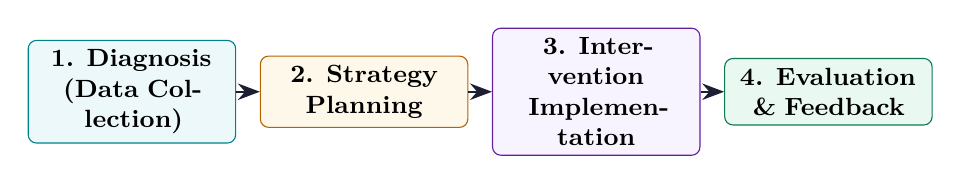
\begin{tikzpicture}[node distance=0.35cm, auto]
  \node [block, fill=hdrteal!50, draw=myteal] (d) {1. Diagnosis\\(Data Collection)};
  \node [block, right=0.3cm of d, fill=hdramber!50, draw=myamber] (s) {2. Strategy\\Planning};
  \node [block, right=0.3cm of s, fill=hdrpurple!40, draw=mypurple] (i) {3. Intervention\\Implementation};
  \node [block, right=0.3cm of i, fill=hdrgreen!60, draw=mygreen] (e) {4. Evaluation\\\& Feedback};

  \draw [arrow] (d) -- (s);
  \draw [arrow] (s) -- (i);
  \draw [arrow] (i) -- (e);
\end{tikzpicture}
\end{tcolorbox}

\subsection{Major OD Interventions}
\par\vspace{6pt}\noindent
\begingroup
\setlength{\tabcolsep}{5pt}%
\setlength{\extrarowheight}{3pt}%
\renewcommand{\arraystretch}{1.35}%
\begin{tabularx}{\linewidth}{|>{\raggedright\arraybackslash\bfseries}p{3.5cm}|Y|}
\hline
\multicolumn{1}{|c|}{\textbf{Intervention Type}} & \multicolumn{1}{c|}{\textbf{Description \& Operational Focus}} \\
\hline
Team Building & Structured activities designed to improve interpersonal trust, goal clarity, and team cohesion. \\
\hline
Sensitivity Training (T-Groups) & Unstructured group interaction sessions aimed at increasing self-awareness and interpersonal sensitivity. \\
\hline
Process Consultation & An outside consultant assists managers in perceiving, understanding, and acting upon process events (e.g., meeting dynamics). \\
\hline
Survey Feedback & Systematic collection of data via questionnaires, followed by feedback sessions to diagnose operational issues. \\
\hline
\end{tabularx}
\endgroup

% ===============================================================================
% QUICK REVISION PAGE
% ===============================================================================
\newpage
\begin{center}
  {\large\bfseries\color{myred} Quick Revision --- Module 4}\\[3pt]
  {\small\color{mydark} Organizational Change \& Development $|$ OE-EC804C}
\end{center}
\vspace{-4pt}
\hrule
\vspace{8pt}

\begin{tcolorbox}[formulabox, title={\textbf{Key Concepts and Metrics at a Glance}}]
\renewcommand{\arraystretch}{1.35}
\begin{tabularx}{\linewidth}{>{\raggedright\arraybackslash\bfseries}p{4.5cm} X}
Lewin's Change Model & 3-stage process: Unfreezing (break status quo) $\to$ Changing (movement) $\to$ Refreezing (institutionalization). \\[4pt]
Resistance Factors & Individual (fear, habit, economic security) vs. Organizational (structural inertia, threat to power). \\[4pt]
OD Definition & Planned, long-term, culture-focused effort to improve organizational effectiveness. \\[4pt]
OD Process Stages & Diagnosis $\to$ Strategy Planning $\to$ Intervention $\to$ Evaluation. \\[4pt]
OD Interventions & Team Building, Sensitivity Training (T-Groups), Process Consultation, Survey Feedback. \\
\end{tabularx}
\end{tcolorbox}

\begin{tcolorbox}[defbox, title={\textbf{One-Line Definitions for Exam Revision}}]
  \begin{itemize}[leftmargin=*, itemsep=2pt]
    \item \textbf{Unfreezing:} Breaking down the existing status quo to prepare individuals for organizational change.
    \item \textbf{Refreezing:} Reinforcing and institutionalizing new behaviors to make change permanent.
    \item \textbf{Process Consultation:} Intervention where a consultant helps managers observe and act upon internal communication and team dynamics.
    \item \textbf{Structural Inertia:} Built-in organizational mechanisms (rules, structure) that act as barriers to change.
  \end{itemize}
\end{tcolorbox}

\begin{tcolorbox}[exambox, title={\textbf{Frequently Asked / Viva Questions}}]
\begin{enumerate}[leftmargin=*, itemsep=4pt]
  \Q{Define Organizational Change. Distinguish between Reactive and Proactive change.}{Organizational change is the alteration of structures, processes, or culture. Reactive change is triggered by immediate external pressure; Proactive change is planned in advance to capture opportunities.}
  
  \Q{Explain Lewin's 3-Step Model of organizational change.}{The model consists of Unfreezing (breaking the status quo), Changing (moving to the new state), and Refreezing (reinforcing and institutionalizing the change).}
  
  \Q{What are the primary individual causes of resistance to change?}{Fear of the unknown, habit, threat to economic security, anxiety over skill competence, and selective perception.}
  
  \Q{What are the primary organizational causes of resistance to change?}{Structural inertia, limited focus of change, threat to specialized expertise, and threat to established power relationships.}
  
  \Q{List four key strategies for overcoming resistance to change.}{Education and communication, employee participation, managerial facilitation and support, and incentive negotiation.}
  
  \Q{Define Organizational Development (OD). What are its main objectives?}{OD is a planned, long-term, top-management-driven effort to improve organizational effectiveness through culture management. Objectives: build trust, openness, and problem-solving capacity.}
  
  \Q{What are the 4 stages of the OD process?}{Diagnosis (data gathering) $\to$ Strategy Planning $\to$ Intervention Execution $\to$ Evaluation and Feedback.}
  
  \Q{Explain Sensitivity Training (T-Groups) as an OD intervention.}{An unstructured group interaction technique designed to increase self-awareness, empathy, and interpersonal communication skills.}
  
  \Q{What is Survey Feedback in OD?}{A diagnostic intervention where data is collected from employees via questionnaires, analyzed, and presented back to teams to identify operational problems.}
  
  \Q{Why is Team Building considered a critical OD intervention?}{It improves interpersonal trust, role clarity, and communication, transforming individual workers into a cohesive, high-performing team.}
\end{enumerate}
\end{tcolorbox}


\end{document}
